\documentclass{article}
\usepackage[normalem]{ulem}
\usepackage[utf8]{inputenc}
\usepackage{graphicx}
\usepackage{mathtools}
\usepackage{amssymb}
\usepackage{amsmath}
\usepackage{macros}
\usepackage{color}

\begin{document}
\section{Funktionsundersökning}
Givet: en funktion $f(x)$\\
Mål: undersök de väsentliga aspekterna av $f$:s beteende och rita grafen $y=f(x)$\\

\begin{enumerate}
  \item Bestäm definitionsmängden $D_f$ (om den inte redan är given):
man måste undvika division med noll, roten ur negativa tal, etc.
Se up med skillnaden mellan $ln(\cdots)$ och $ln\abs{\cdots}$.

  \item Innan du börjar räkna, tänk efter om det finns några \uline{uppenbara egenskaper}
    som man kan se direkt. (Är funktionen alltid positiv? Jämn/udda (potenser)?
    Kan man se var den har nollställen?
    Approximationer $f(x)=(???), x\approx0$ eller då $\abs x$ är stort?)
    Räkna eventuellt ut några funktionsvärden.

  \item Undersök relevanta gränsvärden för att avgöra om kurva $y=f(x)$ har några \uline{asymptoter}:
  \begin{itemize}
    \item Linjen $x=a$ är en lodrät asymptot om $f(x)\to\infty$ eller $f(x)\to-\infty$ då $x\to a^+$ och/eller $x\to a^{-1}$.\\
      T.ex.\\
      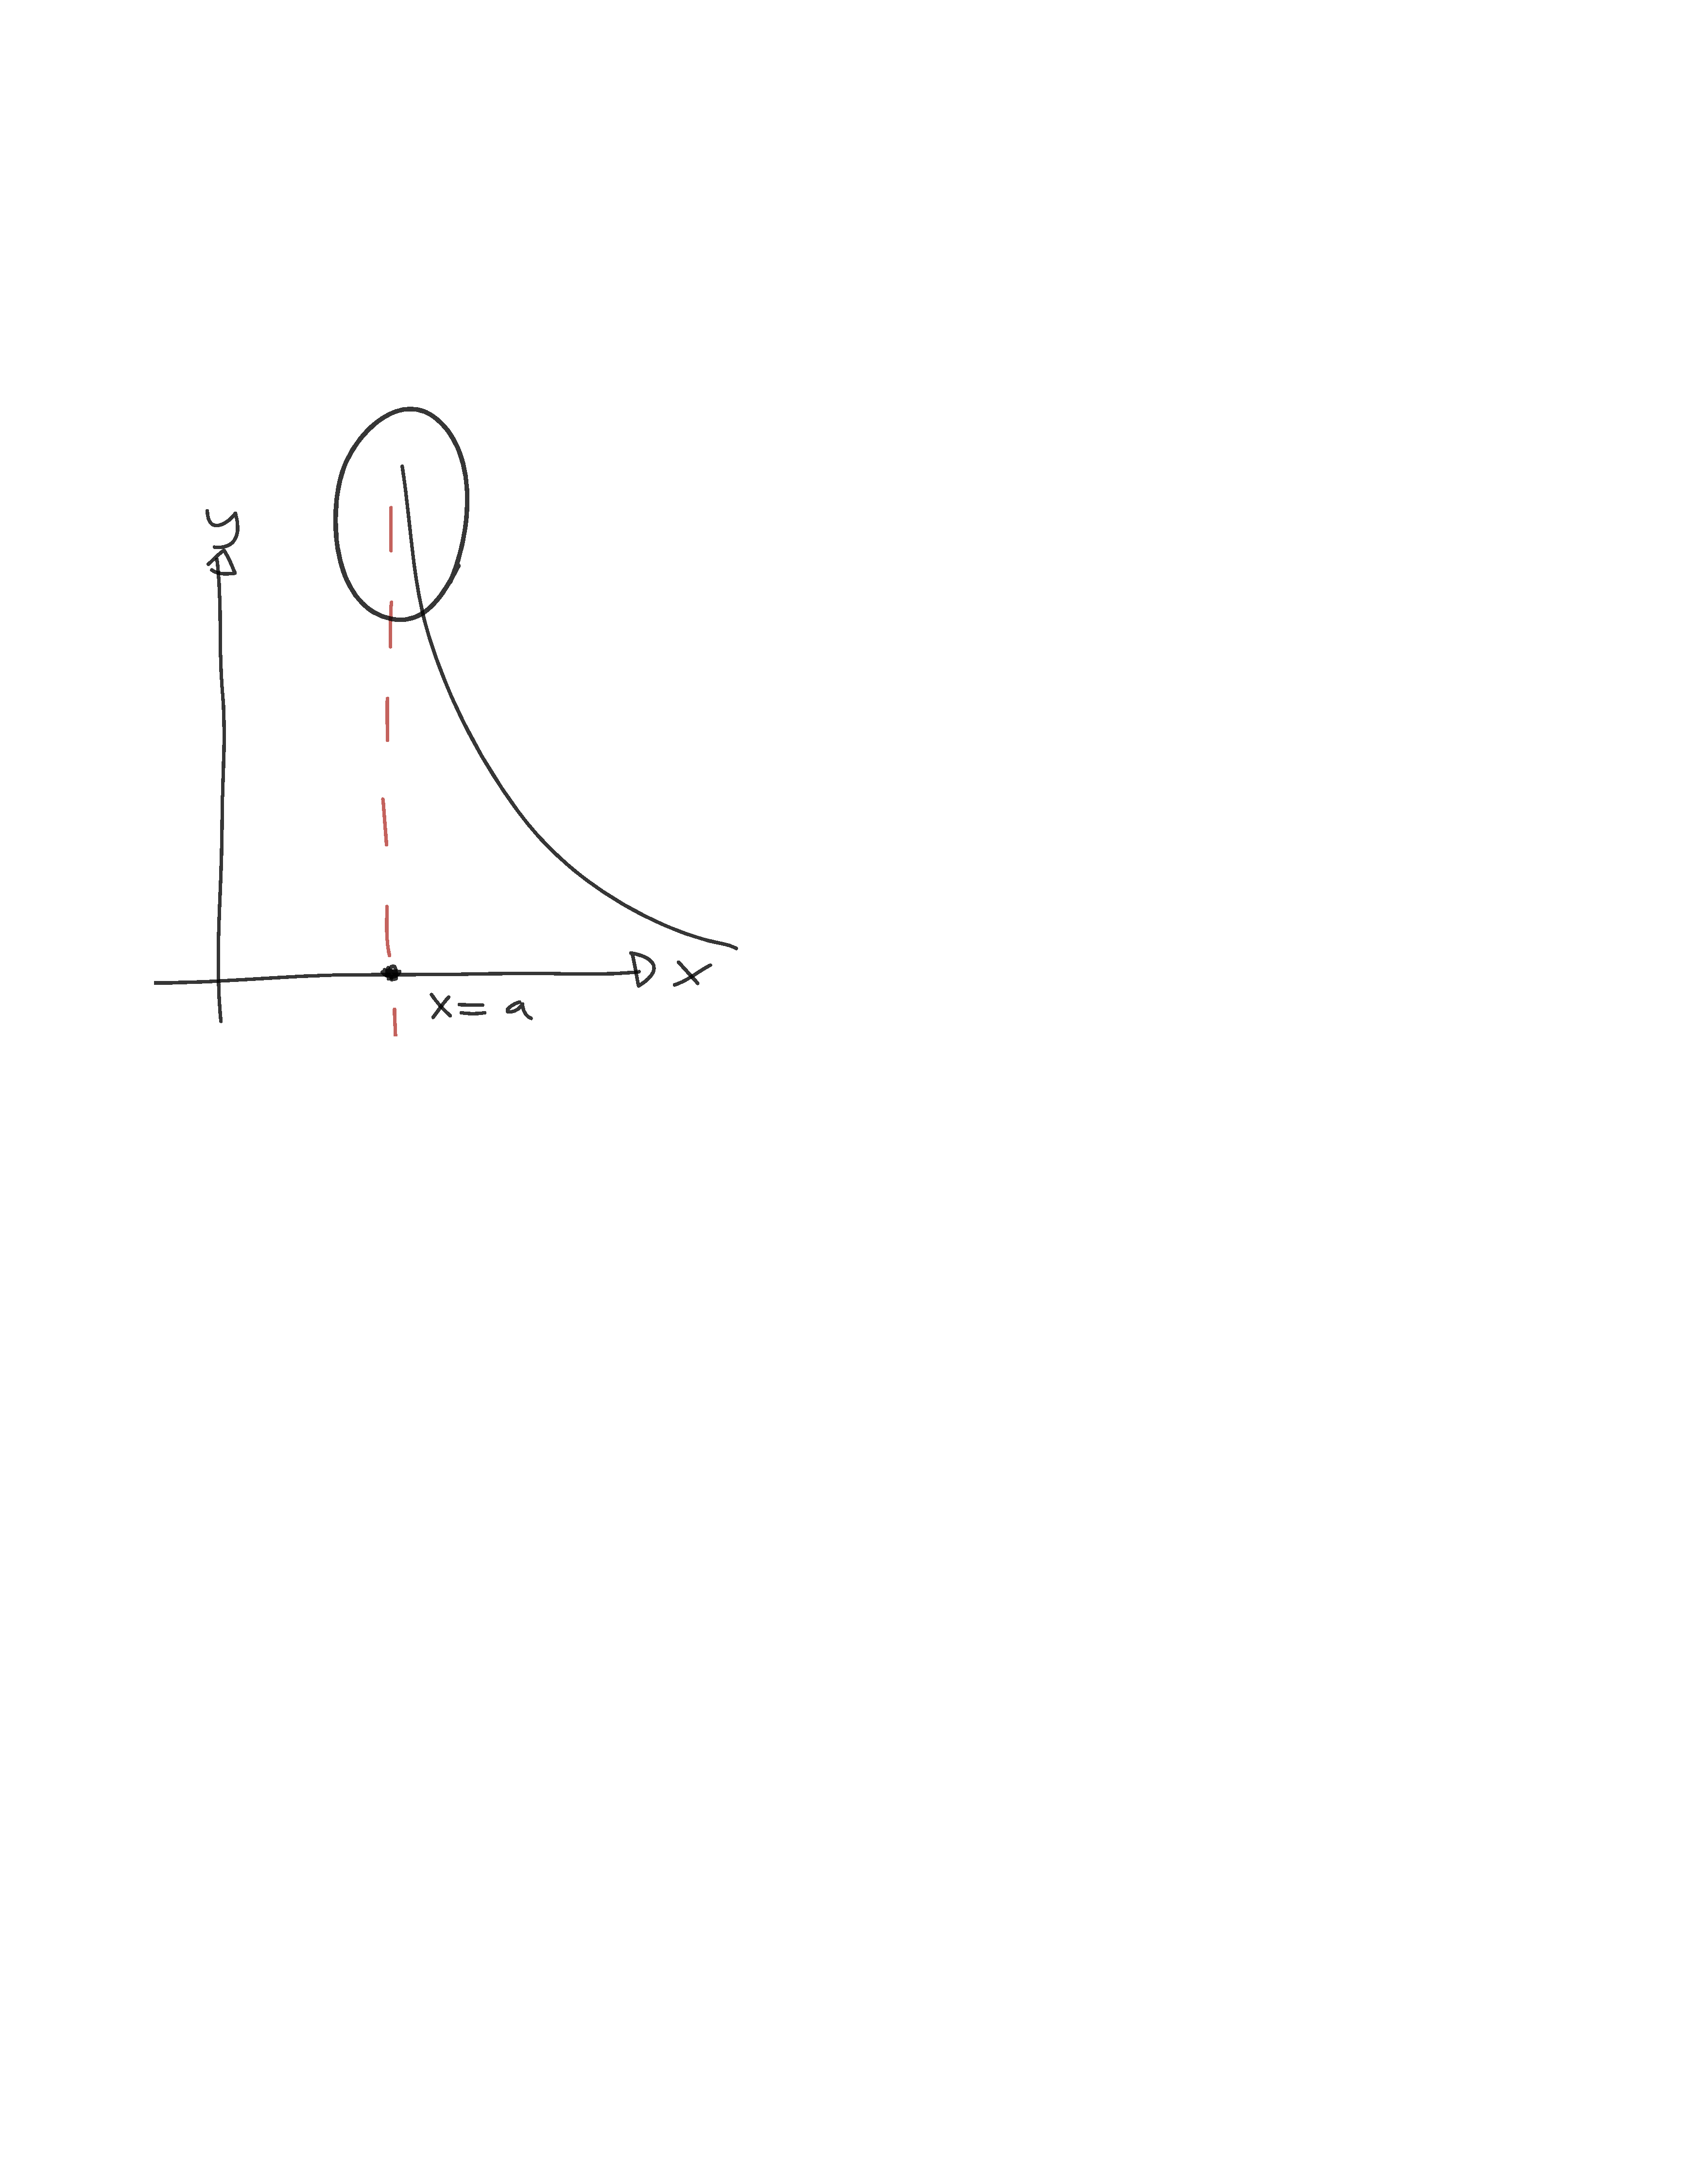
\includegraphics[scale=0.2]{img/asym1.pdf}\\
      (Kan bara hända om $f$ är diskontinuerlig eller odefinerad i punkten a.)
    \item Linjen $y=k$ är en \uline{vågrät asymptot} om $f(x)\to k, x\to\infty$ och/eller då $x\to -\infty$\\
      T.ex.\\
      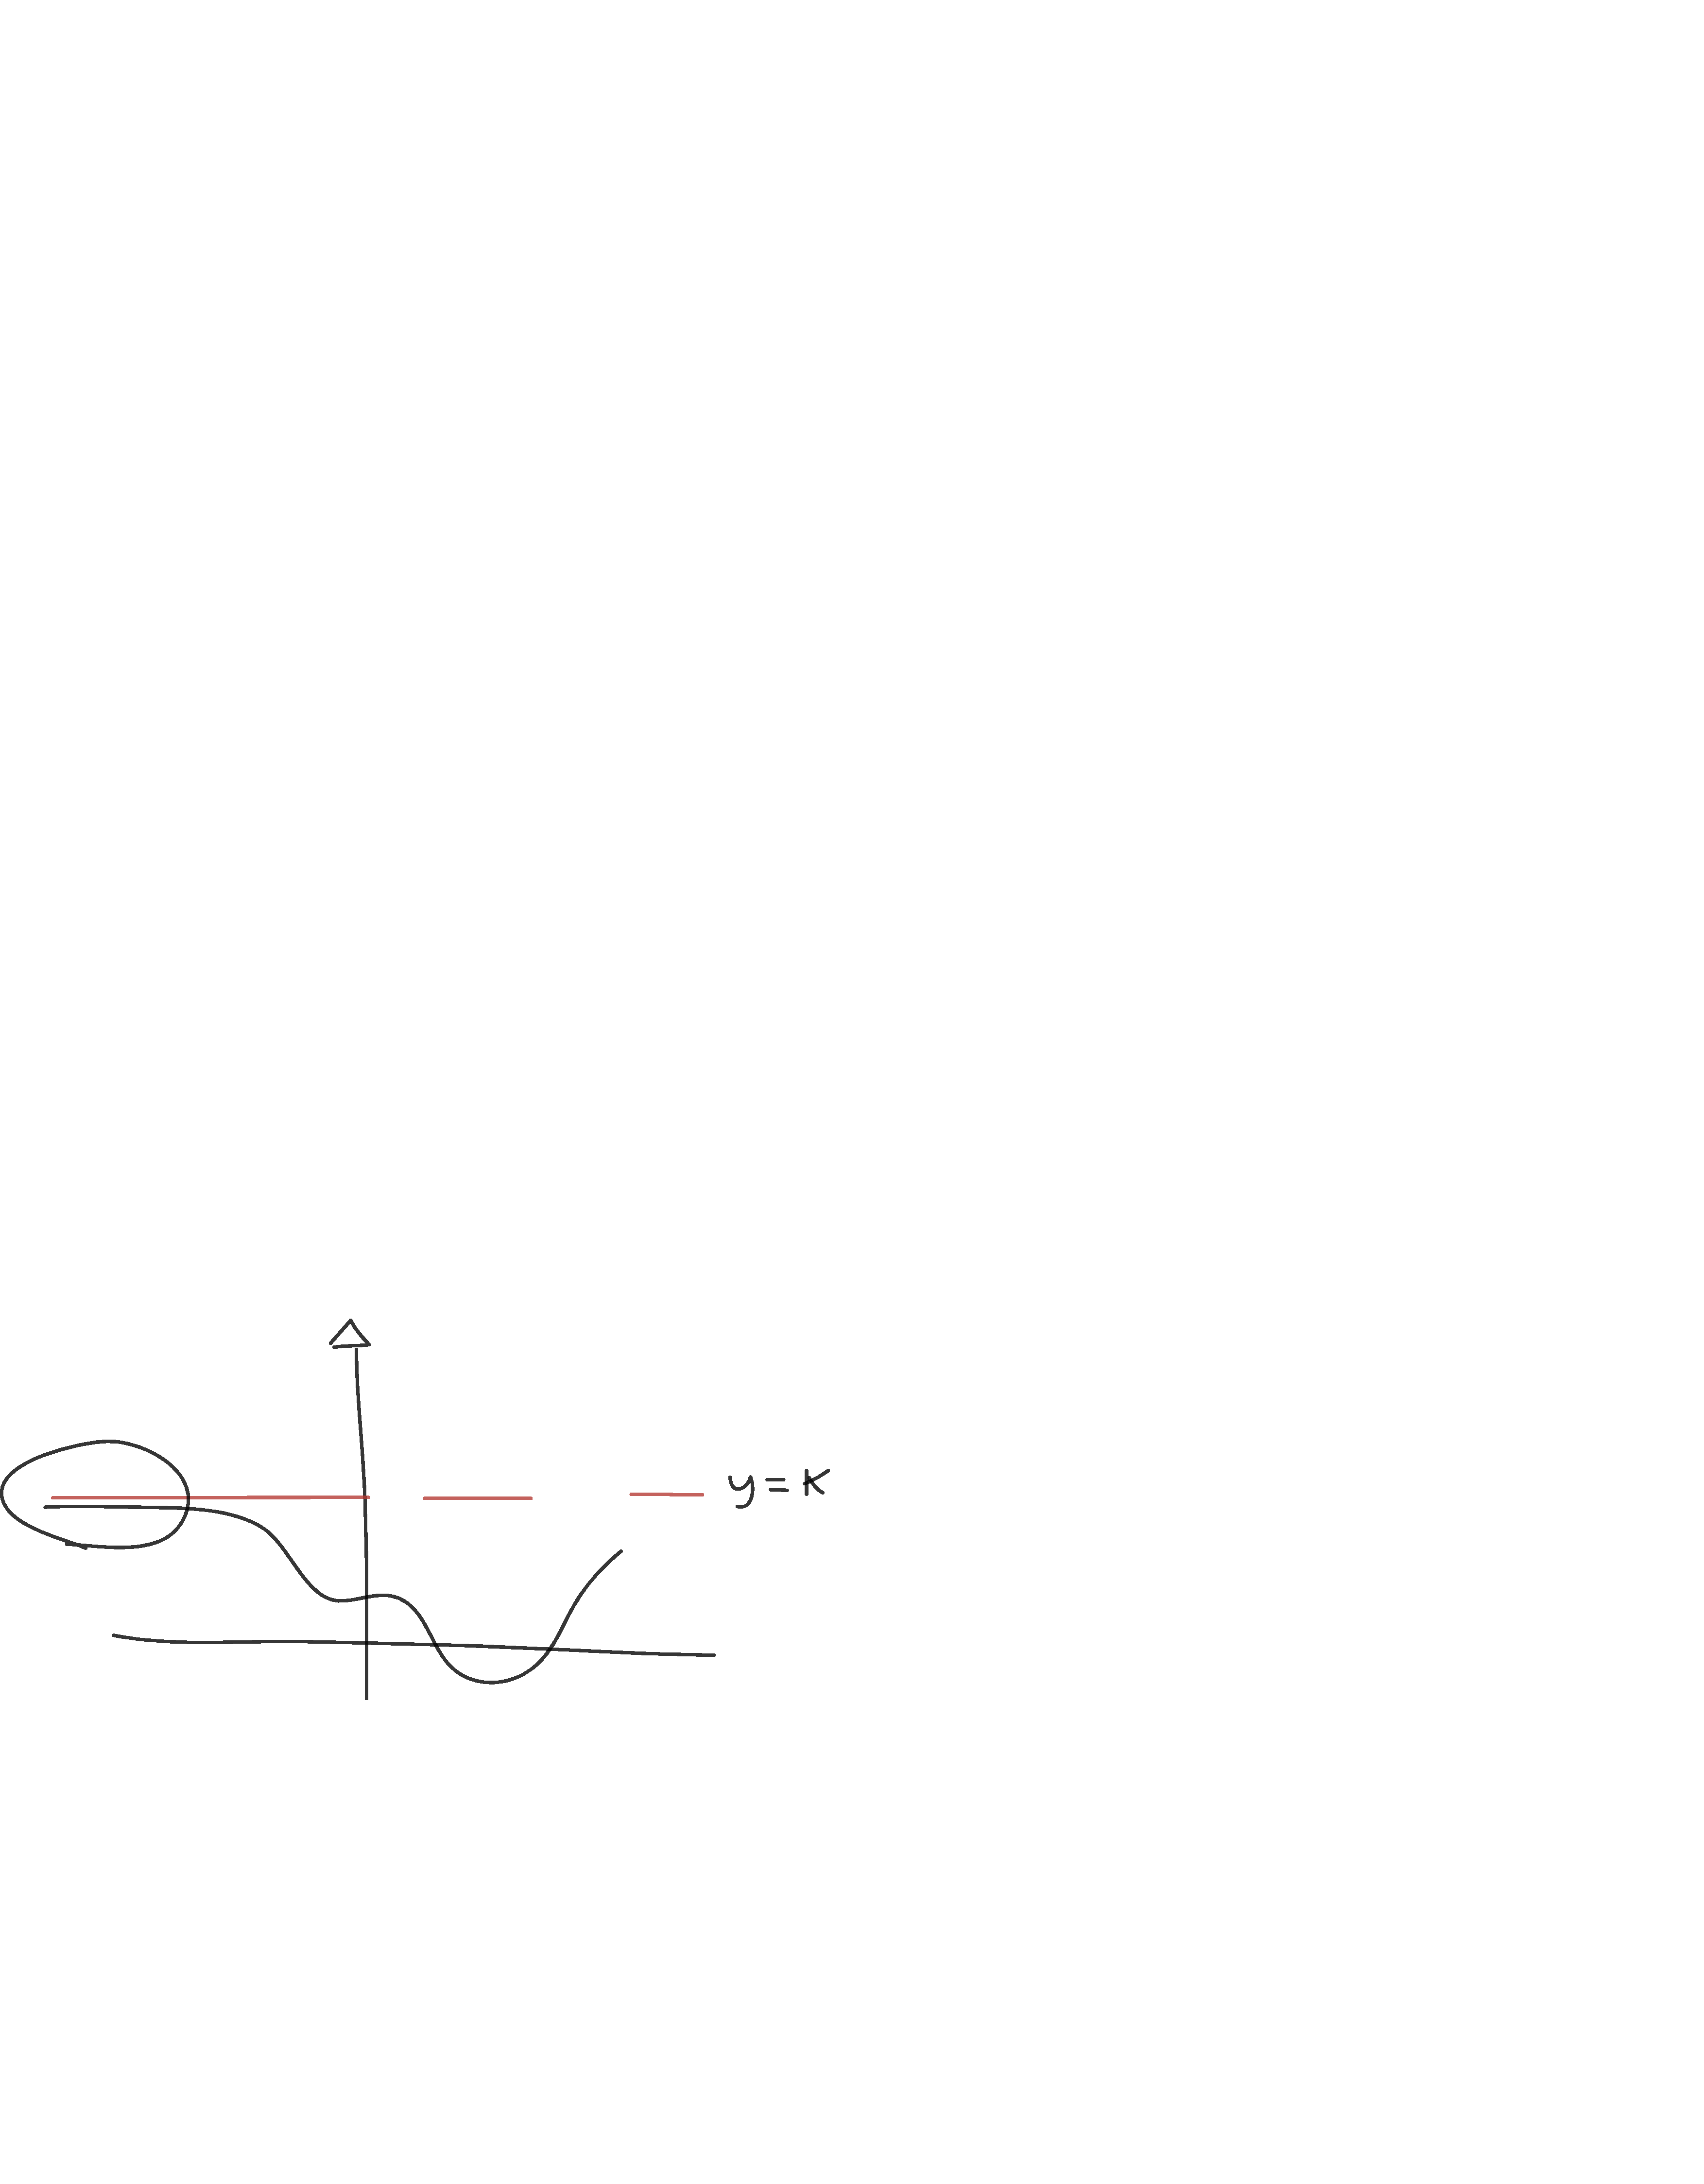
\includegraphics[scale=0.3]{img/asym2.pdf}\\
    \item (Överkurs) $y=kx+m$ är en \uline{sned asymptot} om $f(x)-(kx+m)\to 0, x\to infty$ och/eller $x\to -\infty$\\
      T.ex.\\
      
\includegraphics[scale=0.7]{img/asym3.pdf}\\
      (Undersök $\lim \f{f(x)}{x}$ för att hitta k, sedan $\lim \left(f(x)-kx\right)$ för att hitta m.)
  \end{itemize}

  \item Räkna ut derivatan $f'(x)$, faktorisera så långt som möjligt, och gör sedan en \uline{teckentabell} för att avgöra var $f'$ är positiv/negativ/noll/(odef.)
    (så att man ser var $f$ är växande/avtagande respektive har lokal max/min eller terrasspunkter).

  \item (Överkurs) Gör en funktionsundersökning av $f'$ för att avgöra var funktionen $f$ är \uline{konvex eller konkav}.\\
    $f$ är \uline{kon{\color{red}vex}} på ett intervall $I$ $\eq$ varje sekand i $I$ ligger ovanför grafen $\eq$ $f'$ är {\color{red}väx}ande på $I$ $\eq f'' \ge 0$ på $I$.
    (Konk{\color{red}av}: tvärtom ($f'$ {\color{red}av}tagande))
    
\includegraphics[scale=1.3]{img/sekant.pdf}\\

  \item Rita grafen $y=f(x)$ med hjälp av ovanstående information. (Tänk tillbaka på vad $D_f$ var, så att du inte glömmer att rita någon del av grafen, eller ritar någonting där $f$ är odefinerad.)

  \item  MYCKET VIKTIGT: Kontrollera att allt hänger ihop! (Inga motsägelser får finnas.)

  \item Skriv ett svar där det som efterfrågas i uppgiften klart framgår.
    (Det kan gälla asymptoter, lokala extrempunkter, antalet lösningar till ekvationen $f(x)=0$, värdemängden för $f$, etc)
\end{enumerate}

\section{Exempel}
Undersök $f(x)=\f{x-1}{x+1} e^{-1/x}$\\
$$D_f = \{ x\in\R : x\neq -1, x\neq 0 \}$$
$f$:s enda nollställe är $x=1$, och man kan se $f$:s tecken med en teckentabell.

\begin{tabular}{ l | l l l l l l l }
  $x$   &   & -1&   & 0 &   & 1 &   \\\hline
  $x-1$ & - &   & - &   & - & 0 & + \\
  $x+1$ & - & 0 & + &   & + &   & + \\
  $e^{-1/x}$
        & + &   & + & ~ & + &   & +\\\hline
  $f(x)$& + & ~ & - & ~ & - & 0 & +
\end{tabular}\\

\subsection{Relevanta gränsvärden}
\begin{itemize}
  \item $f(x)=\f{1-1/x}{1+1/x}e^{-1/x} \to \f 11 e^0 = 1, x\to\pm\infty$ så linjen $y=1$ är en vågrät asymptot.
  \item $f(x)=\f{1-x}{1+x}e^{-1/x} \to 0, x\to 0^+$
  \item $f(x)=\f{1-x}{1+x}e^{-1/x} \to -\infty, x\to 0^-$, så linjen $x=0$ är en lodrät asymptot.
  \item $f(x)=\f{1}{x+1}(x-1)e^{-1/x} \to \pm\infty, x\to (-1)^{\pm}$, så linjen $x=0$ är en lodrät asymptot.
\end{itemize}

\subsection{Derivata}
$$ f'(x) = \f{2}{(x+1)^2} e^{-1/x} + \f{x-1}{x+1}e^{-1/x}\f 1{x^2} =
\f{2x^2+(x-1)(x+1)}{x^2(x+1)^2}e^{-1/x}=$$
$$\f{3x^2-1}{x^2(x+1)^2}e^{-1/x} = \f{3(x+\f1{\sqrt 3})(x-\f1{\sqrt 3})}{x^2(x+1)^2}e^{-1/x}$$

\subsection{Teckentabell över derivatan}
\begin{tabular}{ l | l l l p{7mm} l l l p{7mm} l }
  $x$               &   & -1&   &$\f{-1}{\sqrt 3}$&   & 0 &   &$\f{1}{\sqrt 3}$&   \\\hline
  $3e^{-1/x}$       & + &   & + &   & + & $\nexists$ & + &   & + \\
  $x+\f 1{\sqrt{3}}$& - &   & - & 0 & + &   & + &   & + \\
  $x-\f 1{\sqrt{3}}$& - &   & - &   & - &   & - & 0 & + \\
  $x^2(x+1)^2$      & + & 0 & + &   & + & 0 & + &   & + \\\hline
  $f(x)$            & + & $\nexists$ & + & 0 & - & $\nexists$ & - & 0 & + \\
  $f'(x)$           & $\nearrow$ & $\nexists$ & $\nearrow$ & lok. max & $\searrow$  & $\nexists$ & $\searrow$  & lok. min & $\nearrow$
\end{tabular}\\

\subsection{Lokalt maximum}
$$ f(\f{-1}{\sqrt 3}) = \f{\sqrt 3 + 1}{-\sqrt 3 - 1} e^{\sqrt 3} \approx 21.09$$

\subsection{Lokalt minimum}
$$ f(\f{1}{\sqrt 3}) = \f{\sqrt 3 + 1}{\sqrt 3 - 1} e^{-\sqrt 3} \approx -0.047$$

\subsection{Graf}
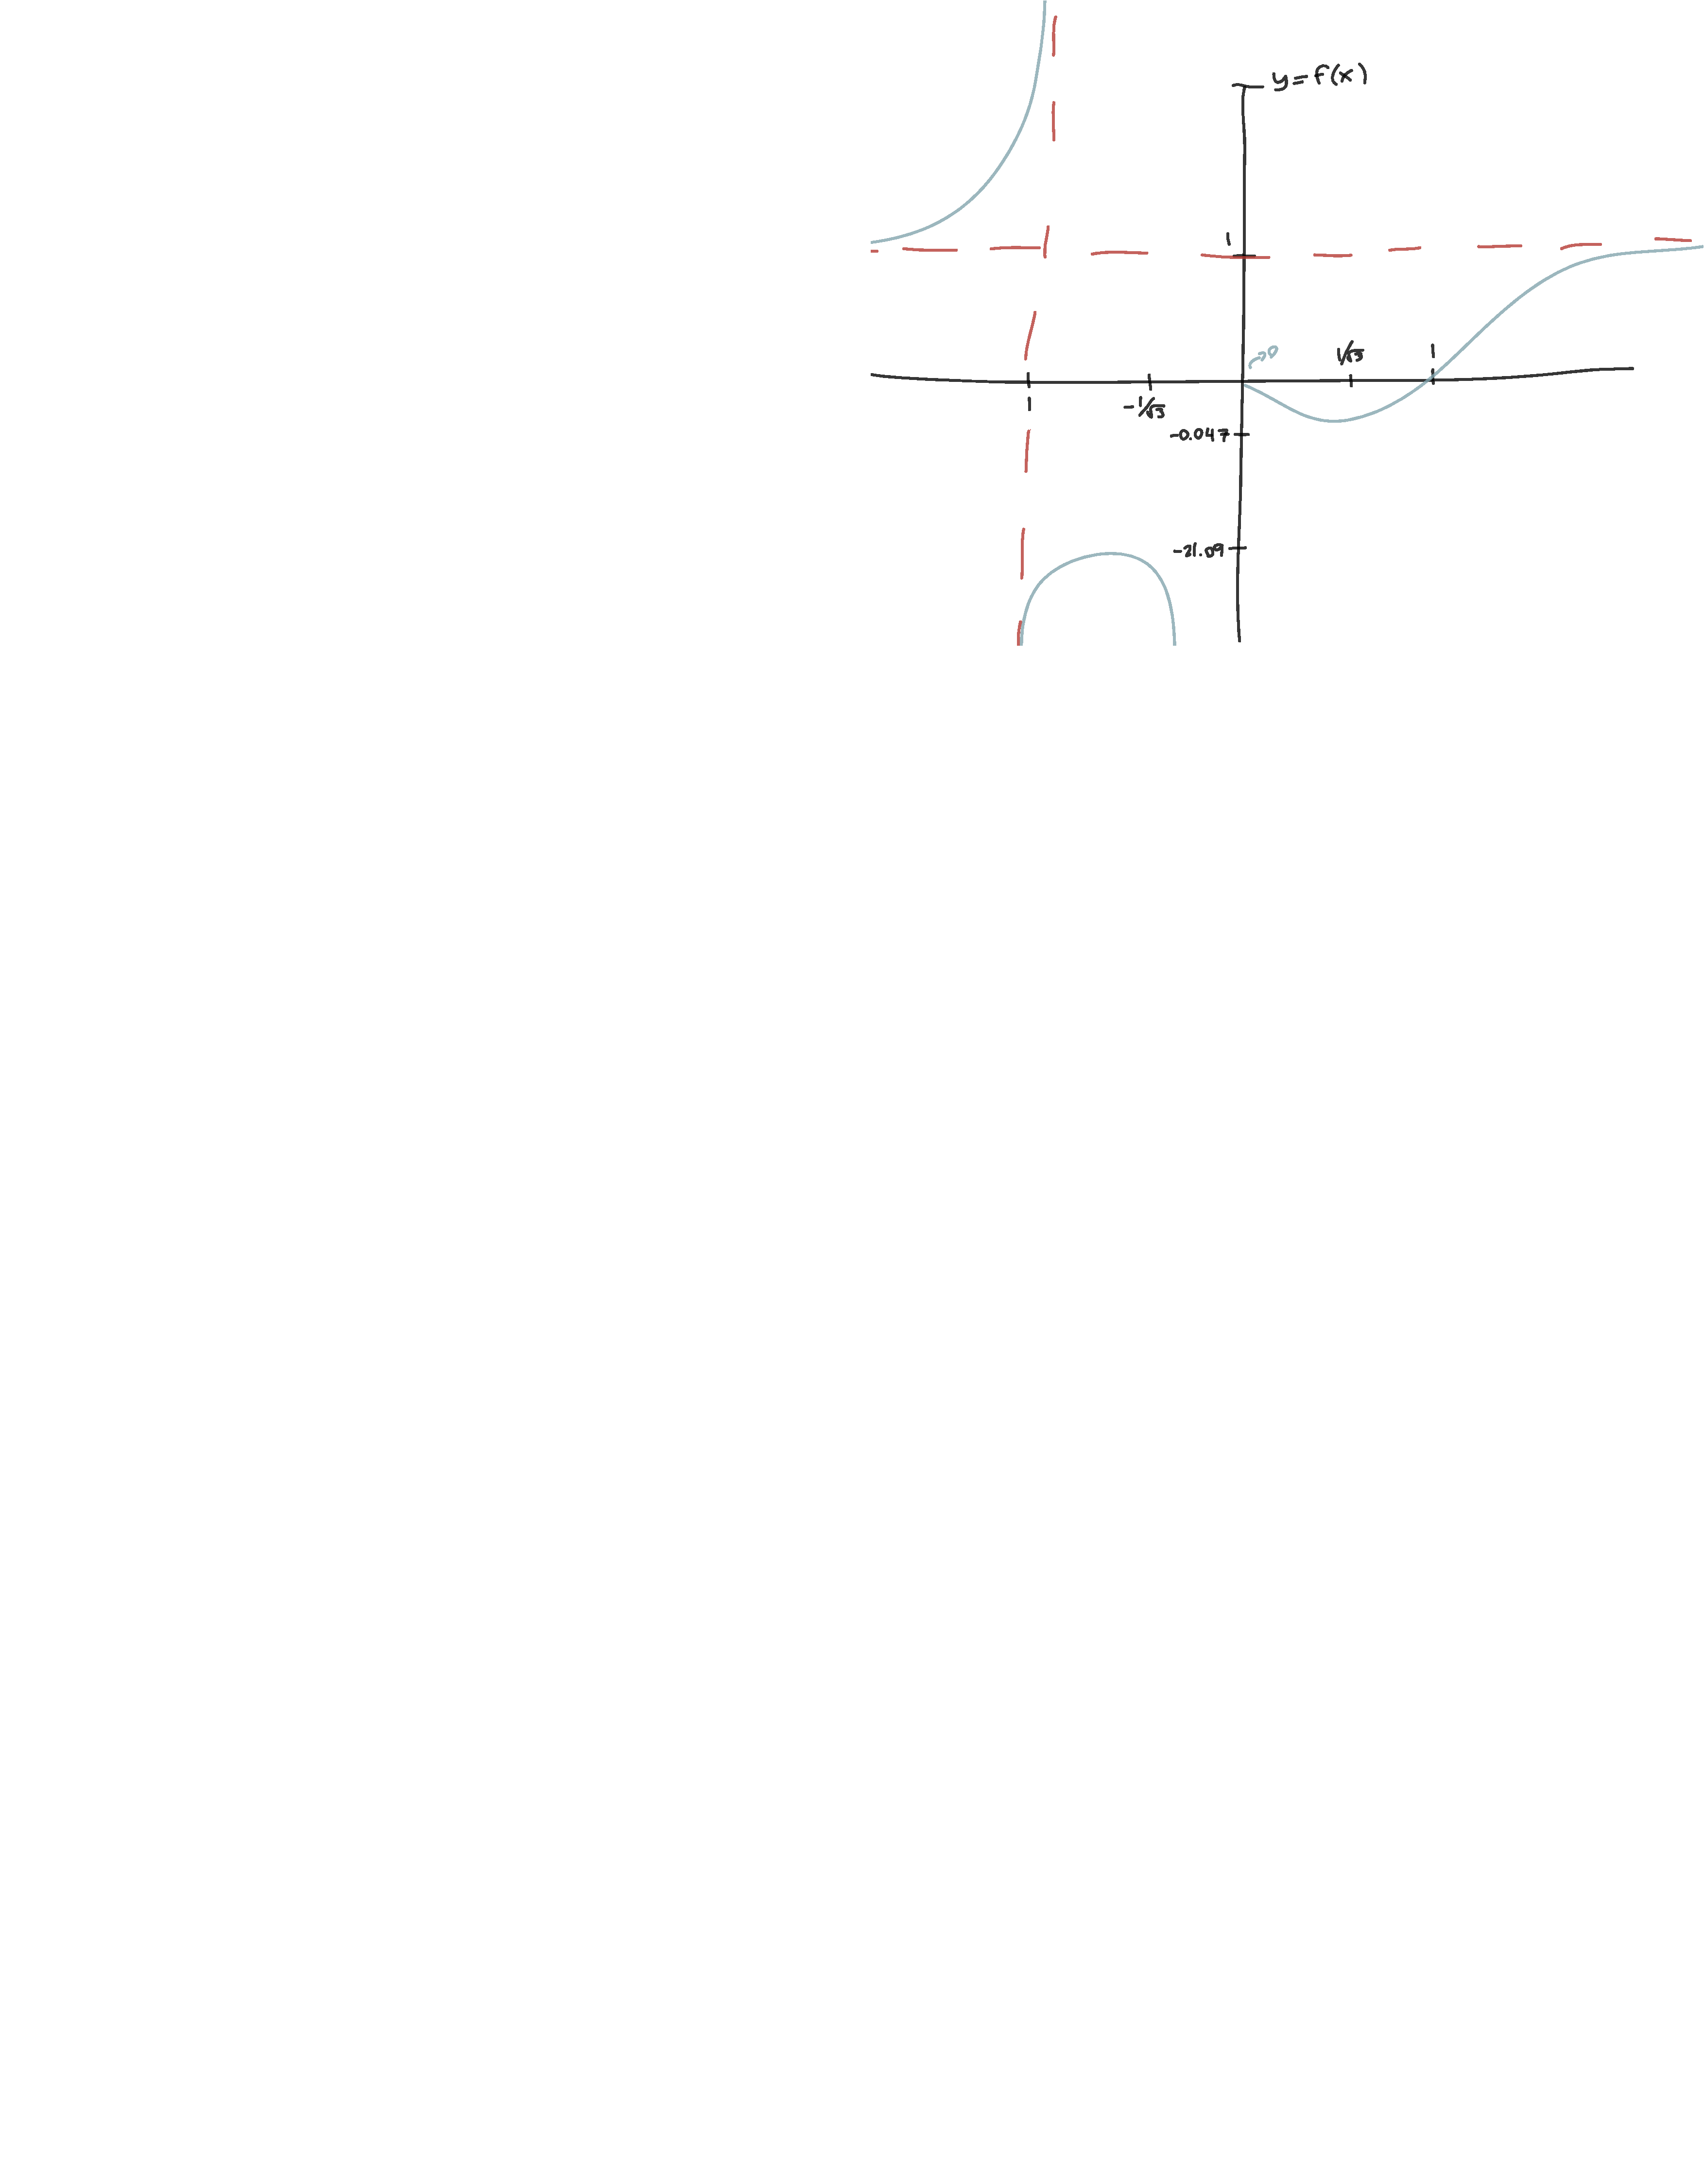
\includegraphics[width=\textwidth]{img/graph.pdf}\\

\end{document}
